\documentclass[conference]{IEEEtran}
% arXiv-ready source. Build: latexmk -pdf main.tex  (or: pdflatex main; pdflatex main)
\usepackage[utf8]{inputenc}
\usepackage[T1]{fontenc}
\usepackage{graphicx}
\usepackage{booktabs}
\usepackage{array}
\usepackage{amsmath}
\usepackage{url}
\usepackage{xcolor}
\usepackage[hidelinks]{hyperref}
\usepackage{microtype}
\graphicspath{{figures/}}
\newcommand{\um}{\,$\mu$m}
\newcommand{\code}[1]{\texttt{#1}}

\title{Where LLM Layout Generation Fails:\\An Open-Source Reproduction of LLM-Driven Template-and-Grid Layout\\and an Interface Layer That Makes It Self-Healing}

\author{\IEEEauthorblockN{Jongkyoung, Han}% <-- replace
\IEEEauthorblockA{Independent researcher\\ \url{https://github.com/Toragonite/laygo2-llm-agent}}}

\begin{document}
\maketitle

\begin{abstract}
You et al.\ (MLCAD 2024 WIP) proposed letting a large language model (LLM) write Python layout generators for the template-and-grid framework LAYGO2 from natural-language instructions, with the designer inspecting the result and asking for modifications. We reproduce this flow on a fully open-source stack (public laygo2, SkyWater SKY130, Magic, netgen) with a scripted DRC/LVS judge, a fixed protocol for the human's instructions, and a failure taxonomy. On eight transistor-level cells (2--11 transistors, including the paper's 2-to-1 MUX, ratioed TSPC flip-flop and strong-arm latch), five attempts each, GPT-4o passes 0 of 40 attempts on the six context turns alone and 21 of 40 after up to eight human instructions. Labelling every failing round shows that most failures are not circuit mistakes but friction at the LLM--framework interface: misused return values, wires on occupied tracks, and a routing primitive that silently fills a rectangle between misaligned points. We add a thin, net-aware layer, \code{laygo2\_safe}, that keeps laygo2's architecture and adds validated inputs, an occupancy table, a \code{connect()} primitive with track search, and netlist-aware checks that fail at the offending line. The same tasks then pass 40 of 40 (13 of 40 on the first turns); fix rounds drop from 225 to 41 and interface-type failure labels from 134/127/85 to 7/5/0. Because every remaining failure is a precise tool message, feeding it back verbatim replaces the human: 40 of 40 pass with no human in the loop (24 of 40 on the first turns, 56 automatic rounds, about \$2.4). Layout area matches the human-written references (ratio 0.98); the automatic router uses more metal2 on the larger cells, which we measure and leave as future work. All logs, prompts and protocols are released.
\end{abstract}

\begin{IEEEkeywords}
layout generation, large language models, LAYGO2, SKY130, design automation, benchmark
\end{IEEEkeywords}

\section{Introduction}
Custom cell layout---logic standard cells and high-speed mixed-signal primitives---is still largely manual. Generator-based frameworks such as BAG and LAYGO/LAYGO2~\cite{bag2,laygo,laygo2} let designers describe a layout as Python code over process-portable templates and abstract grids, which raises productivity but moves the burden to writing that code. You et al.~\cite{you2024} asked whether an LLM can write the generator from natural language, with the designer steering interactively, and reported thirteen DRC/LVS-clean designs, from NAND gates to a 32\,Gb/s serializer, using ChatGPT-4.

Their report leaves questions open for anyone who wants to build on it: the prompt logs are no longer available, the process node and tools are not stated, each design is reported once (no success rate or variance), and the amount of human help is summarized only as a prompt count. This work makes the setting reproducible and measurable, and then uses the measurement to find and fix the bottleneck. Our contributions are:
\begin{enumerate}
\item an open-source reproduction: public laygo2 (pinned), SKY130, Magic DRC and netgen LVS wrapped in a one-command judge that was first validated with human-written reference layouts, including three verification pitfalls that would otherwise produce false passes or false failures (\S\ref{sec:judge});
\item a measurement protocol for interactive LLM layout generation: four specificity levels for the human's instructions, a five-type failure taxonomy applied to every failing round, a cap on instructions, and contamination rules (\S\ref{sec:protocol});
\item a baseline on eight cells $\times$ five attempts (\S\ref{sec:baseline}) and a failure analysis showing that interface friction, not circuit knowledge, dominates (\S\ref{sec:failures});
\item \code{laygo2\_safe}, a thin layer over laygo2 that removes that friction without changing laygo2's architecture (\S\ref{sec:layer}), validated by rewriting all eight reference layouts on it;
\item measurements with the layer under human instructions and under purely automatic feedback (\S\ref{sec:results}), a negative result for one feedback variant, and quality metrics beyond pass/fail (\S\ref{sec:quality}).
\end{enumerate}

\section{Background}
\textbf{Template-and-grid layout.} In LAYGO2 a \emph{template} is a pre-drawn, DRC-clean block (a transistor with a given number of fingers, a via), and a \emph{grid} maps integer coordinates to physical positions whose pitches absorb the process's width and spacing rules. A generator places template instances on a placement grid and draws wires on routing grids by integer track indices; the same code targets another process by swapping the technology file. The abstraction suits an LLM because coordinates are small integers and most design rules are absorbed by templates and grids.

\textbf{The paper's flow.} The LLM first converts a SPICE netlist into per-transistor dictionaries (\code{N0 = \{"D": "O", "G": "A", "S": "INT"\}}); then, over several turns in which the designer explains placement rules, alignment strategy, routing commands and track-based routing strategy, it emits placement and routing code. The designer inspects the layout and issues modification instructions until DRC and LVS pass (Figs.~2--4 of~\cite{you2024}). Reported prompt counts range from 3+3 (NAND) to 9+36 (strong-arm latch). The authors rate interactive placement and routing as good, and autonomous optimization as normal (placement) to bad (routing).

\section{Experimental Setup}
\subsection{Stack}
Table~\ref{tab:stack} lists the components. Later laygo2 versions are incompatible with the SKY130 workspace, so the January 2024 commit is pinned. The public release lacks the \code{netmap} module used by the paper's authors; since the netlist-to-dictionary step is performed by the LLM, it is not needed.

\begin{table}[t]
\caption{Software stack.}
\label{tab:stack}
\centering\footnotesize
\begin{tabular}{@{}p{0.27\columnwidth}p{0.66\columnwidth}@{}}
\toprule
component & version \\
\midrule
laygo2 (public) & commit \code{cc6276a}; SKY130 workspace \code{e7bc4fd} \\
process & SKY130A, open\_pdks \code{6d4d117} \\
DRC / extraction & Magic 8.3.460 (from source), deck \code{drc(full)} \\
LVS & netgen 1.5.133, SKY130 setup \\
LLM (reproduction) & \code{gpt-4o-2024-05-13} \\
LLM (improvement) & \code{gpt-4o-2024-08-06}, prompt caching \\
API settings & provider-default temperature, 4096 output tokens, nothing stored \\
\bottomrule
\end{tabular}
\end{table}

\subsection{Judge and Its Pitfalls}
\label{sec:judge}
\code{flow/check\_cell.py} runs a generator from the workspace root, sources the exported Magic script in a fresh Magic process (one process per cell), runs DRC, extracts a SPICE netlist, runs LVS against a reference netlist and prints one JSON line (\code{gen\_ok}, \code{drc\_errors}, \code{lvs\_match}, area, stage times, raw error text). Before any LLM was involved, human-written reference generators for all eight cells had to pass it. Three pitfalls were found and are handled in the judge:
\begin{itemize}
\item \textbf{LVS false passes.} netgen 1.5.133 prints ``Circuits match uniquely'' when a transistor width is wrong (it adds ``Property errors were found'' elsewhere) and when two top-level pins are swapped (it only marks \code{**Mismatch**} in the pin table). The LVS wrapper passes only when all three conditions hold; negative controls (wrong width, swapped pins, wrong topology) are rejected for every cell.
\item \textbf{DRC counts.} On the hierarchical cell, \code{drc listall count} includes violations of vias and template pieces checked in isolation (17 on a clean inverter). DRC is run with the full deck on a flattened copy of the top cell.
\item \textbf{Hierarchical extraction.} Magic 8.3.460 silently drops a sub-cell whose only direct contents are via arrays from hierarchical extraction, giving DRC-clean layouts that fail LVS. The gate-level references work around it; the cells used here are flat.
\end{itemize}
Reference netlists use the transistor sizes the templates actually draw (nfet\_01v8\_lvt $W=0.5$\um{} and pfet\_01v8 $W=1.0$\um{} per finger, $L=0.15$\um, two fingers), not the $W=1.2/2.4$\um{} of the workspace's example netlists, which the layouts never draw.

\subsection{Tasks}
Six cells come from the workspace examples, patched to a single size and to our output paths: INV, NAND2, NOR2, TINV, NAND3 and a 2-to-1 MUX (2, 4, 4, 4, 6 and 10 transistors). Two come from Fig.~9 of~\cite{you2024} and were drawn for this work: a ratioed TSPC flip-flop (7) and a strong-arm latch (11); both use two fingers per device and are connectivity references only, neither sized nor simulated. The LLM receives only the cell name and the reference netlist with comments stripped and device names renamed \code{XM1, XM2, \ldots} in file order, so that no layout hint leaks through instance names; the same file is the LVS reference. Each cell is attempted five times.

\subsection{Protocol for the Interactive Loop}
\label{sec:protocol}
The context reconstructs the paper's Figs.~2--4 as six user turns (netlist $\rightarrow$ dictionaries; placement rules and alignment strategy; placement code; routing commands; pin access and track strategy; routing and the complete script). No example generator is shown. The modification loop is governed by Table~\ref{tab:protocol}. Instructions were written by four instances of a coding agent (Claude) acting as the designer, two cells each; this differs from the paper's human designer and introduces instructor variance, which we report.

\begin{table}[t]
\caption{Measurement protocol.}
\label{tab:protocol}
\centering\footnotesize
\begin{tabular}{@{}p{0.19\columnwidth}p{0.71\columnwidth}@{}}
\toprule
instruction levels & L1 tool output only; L2 diagnosis; L3 what to change and which API/rule; L4 coordinates, column numbers, routing plans. Baseline allows $\leq$\,L3. \\
failure types & A API misuse; B circuit-reading error (ties, memberships, omissions); C routing conflict/short; D geometry misunderstanding; E spacing. Multiple labels per failing round. \\
budget & $\leq$\,8 instructions per attempt; one instruction = one message. \\
contamination & instructors never open reference generators or layouts; they see the task netlist, the LLM's code and conversation, the judge's outputs and rendered layouts. \\
record & model, temperature, git hash of prompts and tools, attempt, date, instructor, tokens, per-round labels. \\
\bottomrule
\end{tabular}
\end{table}

\section{Reproduction: Baseline Results}
\label{sec:baseline}
Fig.~\ref{fig:pass} (red) and Table~\ref{tab:baseline} give the baseline. No attempt passed on the six context turns alone: 34 of 40 crashed while running (undefined template variables, misread return values, placement helpers applied to pins) and 6 failed LVS. After up to eight instructions, 21 of 40 passed; all cells with ten or more transistors and both high-speed circuits failed every attempt. Total tokens 2.69\,M in / 0.36\,M out, about \$19. The NAND2 vs NOR2 gap (1/5 vs 5/5 on equal-sized cells) is partly instructor variance: the NOR instructor explained template geometry when the model stalled, the NAND instructor did not. We keep both as they are.

\begin{table}[t]
\caption{Baseline (v1): original laygo2 API, \code{gpt-4o-2024-05-13}, human-style instructions $\leq$\,L3, five attempts per cell.}
\label{tab:baseline}
\centering\footnotesize
\begin{tabular}{@{}lccc@{}}
\toprule
cell & passed & mean instr.\ (passed) & paper P/R \\
\midrule
INV & 5/5 & 2.2 & -- \\
TINV & 5/5 & 2.4 & -- \\
NOR2 & 5/5 & 4.6 & 3 / 2 \\
NAND2 & 1/5 & 7.0 & 3 / 3 \\
NAND3 & 5/5 & 4.0 & -- \\
2-to-1 MUX & 0/5 & -- & 8 / 15 \\
TSPC FF & 0/5 & -- & 3 / 11 \\
strong-arm latch & 0/5 & -- & 9 / 36 \\
\bottomrule
\end{tabular}
\end{table}

\begin{figure*}[t]
\centering
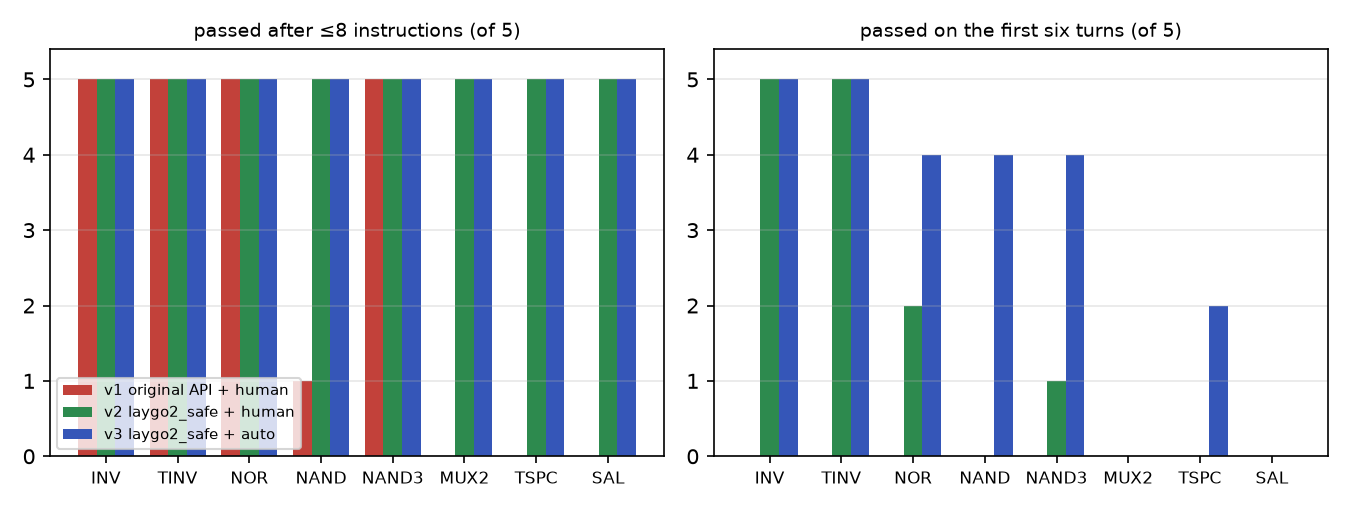
\includegraphics[width=0.9\textwidth]{fig_pass.png}
\caption{Passed attempts per cell (left) and attempts that passed on the first six turns (right), for the three conditions.}
\label{fig:pass}
\end{figure*}

\section{Failure Analysis}
\label{sec:failures}
Every failing round carries one or more labels (Fig.~\ref{fig:labels}). Three interface-type labels dominate the baseline: A (134), C (127) and D (85); B (79) and E (15) follow. The recurring mechanisms were:
\begin{itemize}
\item \textbf{A.} \code{route()} returns a wire or a list depending on the number of objects; \code{route\_via\_track()} returns a list whose last element is the track wire; placement-grid helpers were applied to pins; coordinates taken on one grid were used on another; a two-dimensional placement list with rows of unequal length raises a numpy error (6 of 10 first rounds on the larger cells, and the model regressed to it after fixing it).
\item \textbf{C.} The gate and drain pins of a two-finger template share a column, so the output wire on the drain column shorts the input on the gate column (every inverter attempt); tracks chosen as ``pin\,$\pm$\,1'' land on a neighbour's tied source; a horizontal track on the source row crosses tied sources.
\item \textbf{D.} \code{route()} between two points that differ in both row and column fills the whole rectangle between them, shorting everything underneath (Fig.~\ref{fig:nand}b).
\item \textbf{B.} \code{tie='S'} applied to every transistor regardless of its own dictionary; multi-pin nets built as one nfet drain plus one pfet drain; a transistor dropped from the list when re-ordering.
\end{itemize}
The labels say where to intervene: A, C and D are properties of the tool surface the LLM programs against, not of its circuit knowledge, and B is largely a translation slip from a correct dictionary to code. The netlist-to-dictionary turn was correct in all 40 attempts.

\begin{figure}[t]
\centering
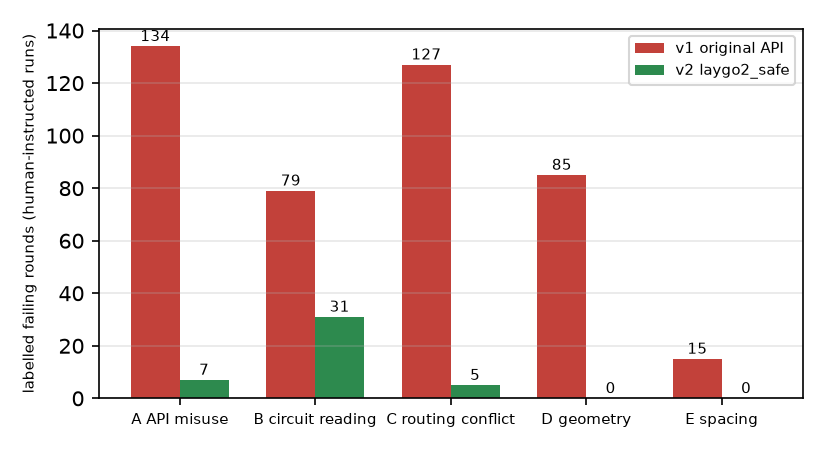
\includegraphics[width=\columnwidth]{fig_labels.png}
\caption{Failure labels over all failing rounds, baseline (v1) versus the interface layer (v2).}
\label{fig:labels}
\end{figure}

\begin{figure*}[t]
\centering
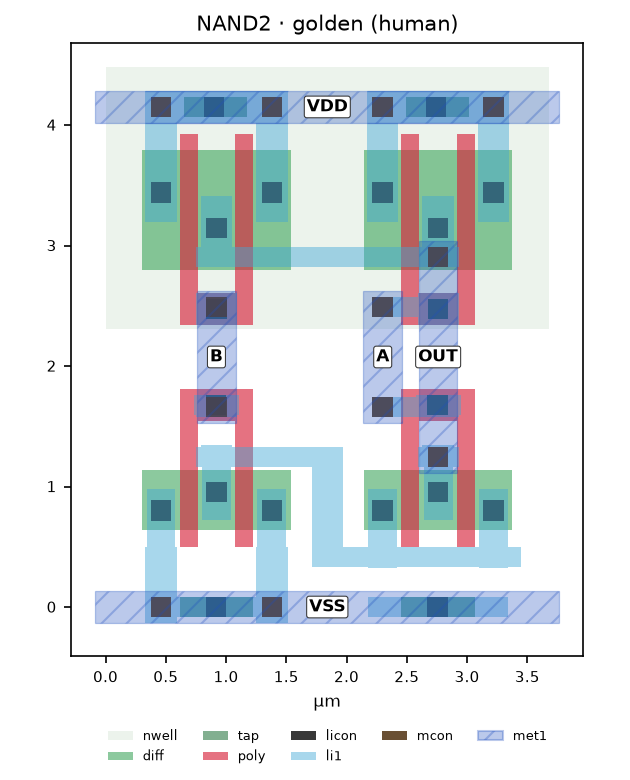
\includegraphics[width=0.32\textwidth]{fig_nand_golden.png}\hfill
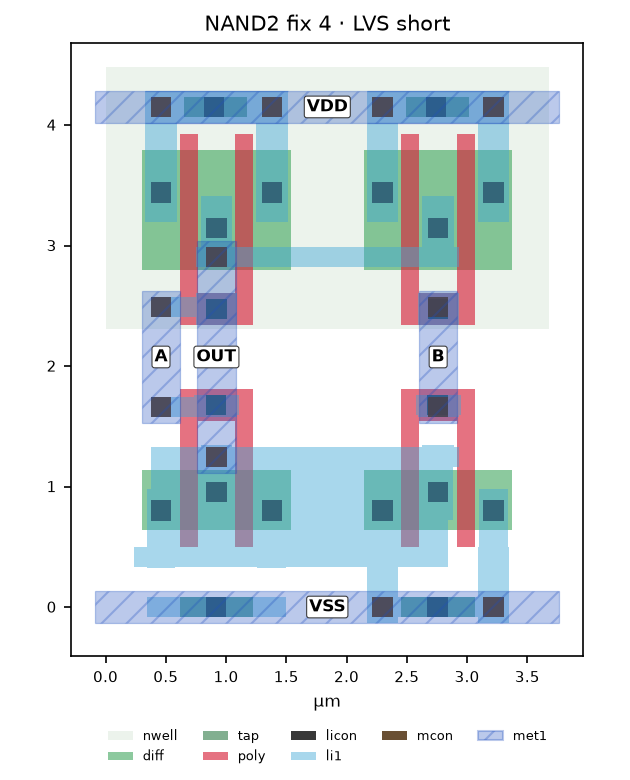
\includegraphics[width=0.32\textwidth]{fig_nand_fail_box.png}\hfill
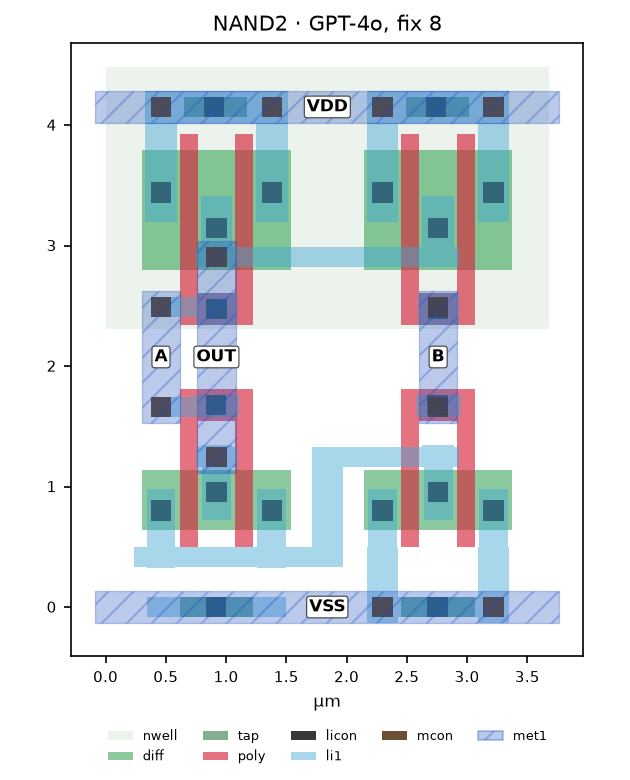
\includegraphics[width=0.32\textwidth]{fig_nand_llm_v1.png}
\caption{NAND2. (a) Human reference. (b) The baseline model after four instructions: DRC-clean but shorted by one \code{route()} call between points on different rows, which fills a rectangle across the nfet row (light blue). (c) The model's passing NAND2 after eight instructions, a mirror image of the reference.}
\label{fig:nand}
\end{figure*}

\section{\code{laygo2\_safe}: A Thin, Net-Aware Layer}
\label{sec:layer}
We kept laygo2's architecture (templates, grids, design database, exporters) and the pinned submodule untouched, and added a layer in the repository that an LLM programs against (Table~\ref{tab:layer}). The cell keeps an \emph{occupancy table} of every pin, wire and via as physical rectangles per layer tagged with a net; pin footprints were measured on the reference layouts (drain strip 0.24\um, source bar $\pm$0.225\um{} past the contacts, gate strap 0.4\um, tied-source straps, via pads $\pm$0.13\um). \code{connect(net, pins, grid)} tries a straight wire, then shared tracks between the pins, then L- and Z-shaped paths, then tracks outside, then an escape on metal2 (grid r34 shares r23's columns); both ends of spanning pins are tried, and a connection with no legal li1 path falls back to metal1. Any geometry that touches another net or is closer than the layer's rule (li1 0.17\um, metal1 0.14\um) is rejected with a message naming the obstacle. Given the reference netlist, \code{nmos(\ldots, ref='XM1')} refuses a wrong tie or finger count at that line, \code{connect()} refuses a pin whose netlist net differs, and \code{check()} lists unconnected pins, wrong nets, missing ports and nets left in separate pieces.

Validation is twofold: 23 guardrail self-tests, and all eight reference cells rewritten on the layer using only \code{connect()} (no coordinates, no track indices) pass DRC\,0 / LVS match; the MUX becomes 16\,\% smaller than the human reference because no spacer cells are needed. The six context turns were rewritten for the new API with the same structure and no example code; the tie rule was reworded to ``decide per device from its own dictionary''.

\begin{table}[t]
\caption{Baseline failures and the layer's response.}
\label{tab:layer}
\centering\footnotesize
\begin{tabular}{@{}p{0.34\columnwidth}p{0.57\columnwidth}@{}}
\toprule
baseline failure & layer behaviour \\
\midrule
return-value shapes, grid mixing, pins vs.\ instances & one kind of return value per function; points remember their grid and are refused on another; inputs validated with messages that say what to do instead \\
rectangle fill between misaligned points & \code{wire()} refuses points not on one track; paths are drawn by \code{connect()} \\
shorts and spacing & occupancy table; rejection of touching or too-close geometry \\
finding a free track & \code{connect()} search: straight, between-pin tracks, L/Z paths, outside tracks, metal2 escape \\
errors found only at LVS & netlist-aware refusals at the offending line; \code{check()} \\
ragged placement lists, unplaced devices & \code{place\_rows()} accepts rows of different length and refuses an unplaced device \\
rails, port labels & \code{rails()}; \code{port()} avoids Magic's label collision when two pin boxes share a centre \\
\bottomrule
\end{tabular}
\end{table}

\section{Results with the Layer}
\label{sec:results}
\subsection{Human-Style Instructions (v2)}
Same eight cells, five attempts, \code{gpt-4o-2024-08-06}, instructions $\leq$\,L3 by four coding-agent instructors. Thirteen of 40 attempts passed on the six turns alone (INV and TINV 5/5), and 40 of 40 passed after instructions, with 41 fix rounds in total (v1: 225). Labels fell to A\,7, B\,31, C\,5, D\,0, E\,0 (Fig.~\ref{fig:labels}). Nineteen of the 22 instructions were L2 (relaying the tool's message with a one-line explanation); none was L4. The remaining B failures had three forms: a tie set contrary to the device's own dictionary (6 of 10 first rounds on the high-speed cells), multi-pin nets built as a single drain pair (parallel devices and fan-out gates omitted), and one pfet dropped from the placement list when re-ordering. Each was repaired by a single instruction quoting the library's message. Tokens 0.76\,M in (0.58\,M cached) / 0.08\,M out, about \$2. A first formal run was discarded: a library bug drew a rail given as a single pin as a zero-length stub and failed DRC on INV; the library was fixed and all 40 attempts were re-run so that the tool version is uniform.

\subsection{Automatic Feedback Only (v3)}
Because every failure is now a precise message, we replaced the human with an automatic loop: the feedback is the tool output only (the last traceback line or \code{SafeError}, the script's \code{CHECK:} lines, DRC rule names with boxes, netgen's net/device counts and pin mismatches, the extracted netlist) followed by a fixed sentence asking for the corrected script; at most eight rounds. The library had meanwhile received the four defects found by the v2 instructors (port label layer, unplaced-device message, split-net check, \code{rails()}), so v3 is not the same tool version as v2. Table~\ref{tab:three} and Fig.~\ref{fig:rounds} summarize. Small cells now pass on the first turns (NAND2, NAND3, NOR2 four of five). The larger cells need two to three times more automatic rounds than human rounds (MUX 3.4 vs 1.0, strong-arm latch 5.2 vs 2.8) but all pass within the budget, at zero human time. Fig.~\ref{fig:sal} shows a strong-arm latch produced on the layer.

\textbf{A negative result.} The automatic loop sometimes oscillates between a crash and an LVS mismatch. A feedback variant that appends the history of problems (open / fixed / back again) was tried on paired copies of the ten MUX and strong-arm first-round states: rounds went from 43 to 42 and one attempt failed. The variant is not used.

\begin{table*}[t]
\caption{Three conditions, 8 cells $\times$ 5 attempts.}
\label{tab:three}
\centering\small
\begin{tabular}{@{}llllcccrr@{}}
\toprule
condition & API & repair & passed & first-turn passes & fix rounds & tokens in / cached / out & cost \\
\midrule
v1 & laygo2 & human $\leq$\,L3 & 21/40 & 0/40 & 225 & 2.69\,M / 0 / 0.36\,M & $\approx$\,\$19 \\
v2 & laygo2\_safe & human $\leq$\,L3 & 40/40 & 13/40 & 41 & 0.76\,M / 0.58\,M / 0.08\,M & $\approx$\,\$2 \\
v3 & laygo2\_safe (+fixes) & automatic, L1 & 40/40 & 24/40 & 56 & 0.95\,M / 0.75\,M / 0.10\,M & $\approx$\,\$2.4 \\
\bottomrule
\end{tabular}
\end{table*}

\begin{figure}[t]
\centering
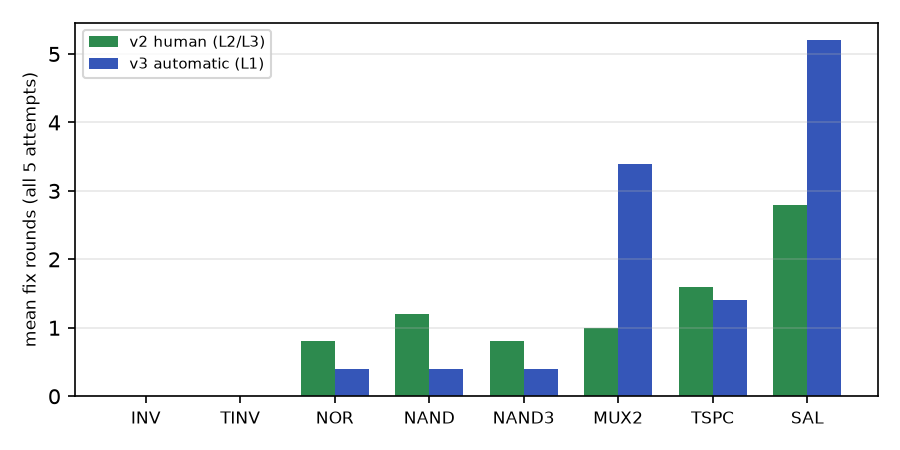
\includegraphics[width=\columnwidth]{fig_rounds.png}
\caption{Mean fix rounds per cell, human instructions (v2) versus automatic feedback (v3), all five attempts.}
\label{fig:rounds}
\end{figure}

\begin{figure}[t]
\centering
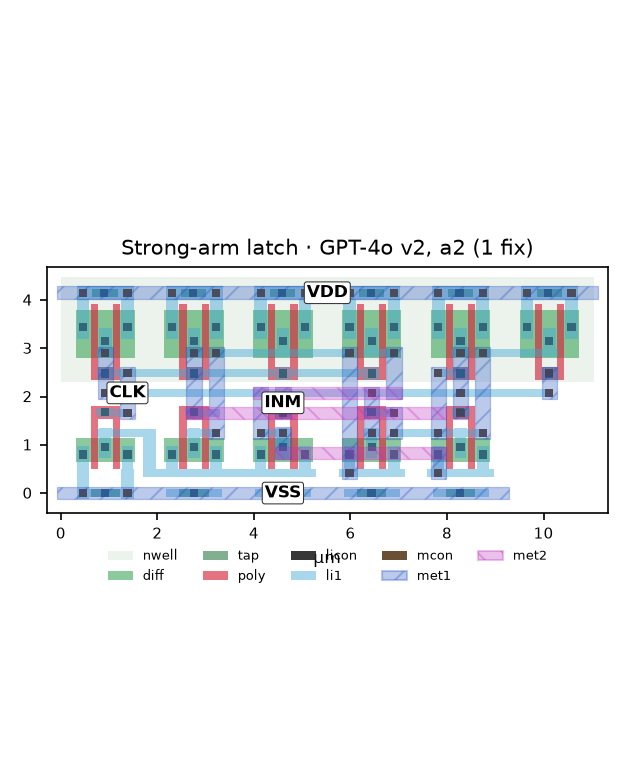
\includegraphics[width=0.8\columnwidth]{fig_sal_llm_v2.png}
\caption{A strong-arm latch produced by the model on the layer, one instruction after the first turns (v2). The baseline model never got this cell past the crash stage.}
\label{fig:sal}
\end{figure}

\section{Quality Beyond Pass/Fail}
\label{sec:quality}
For the 117 passing layouts (8 references, 21 v1, 40 v2, 40 v3) we measured the cell bounding box, the union area of li1, metal1 and metal2 (converted to a length proxy by the minimum width) and contact counts on the flattened layout. Area equals the reference or is smaller (mean ratio 0.98; MUX 16\,\% smaller). li1\,+\,metal1 length is within $\pm$5\,\% for the small cells. On the larger cells the automatic router uses more metal2 than the human designer (strong-arm latch 26\um{} reference, 42\um{} v2, 61\um{} v3; Fig.~\ref{fig:metal2}): when the local-interconnect search fails it escapes upward, where a designer found a lower-layer route. This is the measurable gap between a correct layout and a good one, and the comparison point for the next iteration.

\begin{figure}[t]
\centering
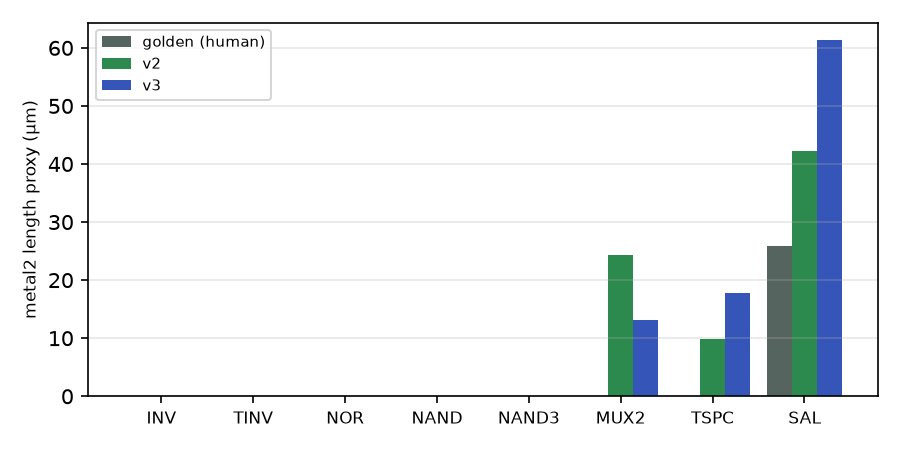
\includegraphics[width=\columnwidth]{fig_metal2.png}
\caption{Metal2 length proxy per cell: human reference versus the layer under human instructions (v2) and automatic feedback (v3).}
\label{fig:metal2}
\end{figure}

\section{Threats to Validity}
\textbf{Confounded changes.} Between v1 and v2 the model (05-13 $\rightarrow$ 08-06, for prompt caching), the library and the prompt wording changed together; between v2 and v3 the library and prompts changed as well as the repair mechanism. The clearest evidence for the library effect is qualitative: during development, the same LLM code went from fail to pass after a library fix alone (NOR, TSPC, strong-arm latch). A control run (same library, human instructions) would separate the feedback effect.
\textbf{Instructor.} Instructions came from coding-agent instances, not an expert designer; help differed between instructors. A pilot run that used L4 instructions was excluded from the baseline.
\textbf{Comparison with the paper.} The paper does not state how prompts were counted, the process, success rates or manual edits (it mentions manual adjustments for the level shifter). Our prompt totals (six context turns plus instructions) are not directly comparable.
\textbf{Scope.} Eight transistor-level cells with at most eleven transistors, two fingers per device; the high-speed cells are connectivity references only; gate-level cells (latch, D flip-flop) have reference layouts but were not benchmarked; five attempts per condition.
\textbf{Tooling.} The judge, the layer and the loops were implemented with a coding agent; all design decisions are logged with reasons in the repository.

\section{Related Work}
Generator-based layout frameworks~\cite{bag2,laygo,laygo2} provide the programmable substrate; rule- and template-based analog layout automation (e.g.\ ALSYN, ALIGN) targets the same cells by other means. LLMs for chip design have mostly produced HDL; You et al.~\cite{you2024} were among the first to generate layout generator code interactively. Our contribution is orthogonal to the model: a measurement protocol and an interface layer that turn the model's failures into messages a loop can act on.

\section{Conclusion}
Reproduced on an open-source stack, the paper's interactive LLM layout flow passes 21 of 40 attempts on eight small cells, and none without human help. Labelling every failure shows that the bottleneck is the interface between the LLM and the framework, not circuit knowledge. A thin net-aware layer that validates inputs, tracks occupancy and finds free tracks removes that bottleneck: 40 of 40 with human help, and 40 of 40 with no human when the layer's messages are fed back verbatim. The remaining gaps are quality (more metal2 than a designer would use) and scale (larger and gate-level cells), both now measurable.

\section*{Reproducibility}
Pinned submodules, the judge, prompts, the protocol, instructor briefs, per-attempt logs (prompts, replies, generated code, DRC/LVS outputs, labels) and CSV summaries are at \url{https://github.com/Toragonite/laygo2-llm-agent}. Runs are tagged \code{20260930} (v1), \code{v2\_20260930} (v2), \code{v3\_selfheal} (v3) and \code{v3b\_selfheal} (feedback variant).

\begin{thebibliography}{9}
\bibitem{bag2} E. Chang et al., ``BAG2: A process-portable framework for generator-based AMS circuit design,'' in \emph{Proc.\ IEEE CICC}, 2018.
\bibitem{laygo} J. Han, W. Bae, E. Chang, Z. Wang, B. Nikoli\'c, and E. Alon, ``LAYGO: A template-and-grid-based layout generation engine for advanced CMOS technologies,'' \emph{IEEE Trans.\ Circuits Syst.\ I}, vol.~68, no.~3, pp.~1012--1022, 2021.
\bibitem{laygo2} T. Shin et al., ``LAYGO2: A custom layout generation engine based on dynamic templates and grids for advanced CMOS technologies,'' \emph{IEEE Trans.\ Comput.-Aided Design Integr.\ Circuits Syst.}, vol.~42, no.~12, pp.~4402--4412, 2023.
\bibitem{you2024} G. You, Y. Byun, S. Lim, and J. Han, ``Interactive and automatic generation of primitive custom circuit layout using LLMs,'' MLCAD 2024 WIP, arXiv:2408.07279, 2024.
\end{thebibliography}

\end{document}
